\documentclass[aspectratio=169,xcolor={dvipsnames,table}]{beamer}
\usepackage[no-math,deluxe,haranoaji]{luatexja-preset}
\renewcommand{\kanjifamilydefault}{\gtdefault}
\renewcommand{\emph}[1]{{\upshape\bfseries #1}}
\usetheme{metropolis}
\metroset{block=fill}
\setbeamertemplate{navigation symbols}{}
\setbeamertemplate{blocks}[rounded][shadow=false]
\usecolortheme[rgb={0.7,0.2,0.2}]{structure}
%%%%%%%%%%%%%%%%%%%%%%%%%%
%% Change alert block colors
%%% 1- Block title (background and text)
\setbeamercolor{block title alerted}{fg=mDarkTeal, bg=mLightBrown!45!yellow!45}
\setbeamercolor{block title example}{fg=magenta!10!black, bg=mLightGreen!70}
%%% 2- Block body (background)
\setbeamercolor{block body alerted}{bg=mLightBrown!25}
\setbeamercolor{block body example}{bg=mLightGreen!15}
%%%%%%%%%%%%%%%%%%%%%%%%%%%
%%%%%%%%%%%%%%%%%%%%%%%%%%%
%% さまざまなアイコン
%%%%%%%%%%%%%%%%%%%%%%%%%%%
%\usepackage{fontawesome}
\usepackage{fontawesome5}
\usepackage{figchild}
\usepackage{twemojis}
\usepackage{utfsym}
\usepackage{bclogo}
\usepackage{marvosym}
\usepackage{fontmfizz}
\usepackage{pifont}
\usepackage{phaistos}
\usepackage{worldflags}
\usepackage{jigsaw}
\usepackage{tikzlings}
\usepackage{tikzducks}
\usepackage{scsnowman}
\usepackage{epsdice}
\usepackage{halloweenmath}
\usepackage{svrsymbols}
\usepackage{countriesofeurope}
\usepackage{tipa}
\usepackage{manfnt}
%%%%%%%%%%%%%%%%%%%%%%%%%%%
\usepackage{tikz}
\usetikzlibrary{calc,patterns,decorations.pathmorphing,backgrounds}
\usepackage{tcolorbox}
\usepackage{tikzpeople}
\usepackage{circledsteps}
\usepackage{xcolor}
\usepackage{amsmath}
\usepackage{booktabs}
\usepackage{chronology}
\usepackage{signchart}
%%%%%%%%%%%%%%%%%%%%%%%%%%%
%% 場合分け
%%%%%%%%%%%%%%%%%%%%%%%%%%%
\usepackage{cases}
%%%%%%%%%%%%%%%%%%%%%%%%%%
\usepackage{pdfpages}
%%%%%%%%%%%%%%%%%%%%%%%%%%%
%% 音声リンク表示
\newcommand{\myaudio}[1]{\href{#1}{\faVolumeUp}}
%%%%%%%%%%%%%%%%%%%%%%%%%%
%% \myAnch{<名前>}{<色>}{<テキスト>}
%% 指定のテキストを指定の色の四角枠で囲み, 指定の名前をもつTikZの
%% ノードとして出力する. 図には remember picture 属性を付けている
%% ので外部から参照可能である.
\newcommand*{\myAnch}[3]{%
  \tikz[remember picture,baseline=(#1.base)]
    \node[draw,rectangle,line width=1pt,#2] (#1) {\normalcolor #3};
}
%%%%%%%%%%%%%%%%%%%%%%%%%%
%% \myEmph コマンドの定義
%%%%%%%%%%%%%%%%%%%%%%%%%%
%\newcommand{\myEmph}[3]{%
%    \textbf<#1>{\color<#1>{#2}{#3}}%
%}
\usepackage{xparse} % xparseパッケージの読み込み
\NewDocumentCommand{\myEmph}{O{} m m}{%
    \def\argOne{#1}%
    \ifx\argOne\empty
        \textbf{\color{#2}{#3}}% オプション引数が省略された場合
    \else
        \textbf<#1>{\color<#1>{#2}{#3}}% オプション引数が指定された場合
    \fi
}
%%%%%%%%%%%%%%%%%%%%%%%%%%%
%%%%%%%%%%%%%%%%%%%%%%%%%%%
%% 文末の上昇イントネーション記号 \myRisingPitch
%% 通常のイントネーション \myDownwardPitch
%% https://note.com/dan_oyama/n/n8be58e8797b2
%%%%%%%%%%%%%%%%%%%%%%%%%%%
\newcommand{\myRisingPitch}{
\begin{tikzpicture}[scale=0.3,baseline=0.3]
\draw[->,>=stealth] (0,0) to[bend right=45] (1,1);
\end{tikzpicture}
}
\newcommand{\myDownwardPitch}{
\begin{tikzpicture}[scale=0.3,baseline=0.3]
\draw[->,>=stealth] (0,1) to[bend left=45] (1,0);
\end{tikzpicture}
}
%%%%%%%%%%%%%%%%%%%%%%%%%%%%
%\AtBeginSection[%
%]{%
%  \begin{frame}[plain]\frametitle{授業の流れ}
%     \tableofcontents[currentsection]
%   \end{frame}%
%}

\usepackage{pxrubrica}
\usetikzlibrary{tikzmark}
%%%%%%%%%%%%%%%%%%%%%%%%%%%
\title{English is fun.}
\subtitle{I will give you some flowers.}
\author{}
\institute[]{}
\date[]

%%%%%%%%%%%%%%%%%%%%%%%%%%%%
%% TEXT
%%%%%%%%%%%%%%%%%%%%%%%%%%%%
\begin{document}


\begin{frame}[plain]
  \titlepage
\end{frame}


\section*{授業の流れ}
\begin{frame}[plain]
  \frametitle{授業の流れ}
  \tableofcontents
\end{frame}
%%%%%%%%%%%%%%%%%%%%%%%%%%%%%
 \section{give \textipa{/g\'Iv/}}
\begin{frame}[plain]{give $+$ 人 $+$ もの}
 \begin{enumerate}
  \item<1-> Birds sing. (SV)
  \item<2-> They speak English. (SVO)
  \item<3-> Cows \textbf{give} us milk. (SVOO)
 \end{enumerate}

\begin{block}<4->{Topics for Today}\small
 \textbf{give}(与える)は目的語を2つとります
\begin{itemize}\setbeamertemplate{items}[square]\small
 \item \textbf{give} $+$ \tikzmark{aa}\Circled[fill color = white]{\,人\,} $+$ \tikzmark{bb}\Circled[fill color = white]{\,もの\,}\hspace{20pt}「\ldots{}に~をあげる」\\
\hfill\tikzmark{AA}{\scriptsize 間接目的語}\\
\hfill\tikzmark{BB}{\scriptsize 直接目的語}
 \item<5-> \begin{tblr}{
         colspec=llll,
         row{1} = {bg=azure3, fg=white},
         row{2} = {bg=white},
         baseline=c,
         hline{1,Z} = {0.08em},
         hline{2} = {0.05em}
}
原形&過去形&過去分詞&ing\\
give \textipa{/g\'Iv/}&gave \textipa{/g\'aIv/}&given \textipa{/g\'Ivn/}&giving \textipa{/g\'IvIN/}
       \end{tblr}
\end{itemize}
\end{block}

\begin{tikzpicture}[remember picture,overlay]
 \visible<4->{\draw[<-] ([xshift=9pt,yshift=-4pt]pic cs:aa) |- ([xshift=-2pt, yshift=2pt] pic cs:AA);}
 \visible<4->{\draw[<-] ([xshift=14pt,yshift=-4pt]pic cs:bb) |- ([xshift=-2pt, yshift=2pt] pic cs:BB);}
\end{tikzpicture}
\hfill{\scriptsize \myaudio{./audio/052_svoo_01.mp3}}
\end{frame}
%%%%%%%%%%%%%%%%%%%%%%%%%%%%%%%%%%
\begin{frame}[plain]{Exercises}

{\small 日本語の意味になるようカッコ内の語句を並べかえましょう。
文頭の語は大文字で始めてください}%
\mbox{}\hfill{\scriptsize \myaudio{./audio/052_svoo_02.mp3}}

 \begin{enumerate}
  \item {\small わたしは彼におもちゃをあげよう。} ( will / him / toy / I / give / a )\\
\visible<2->{I will give him a toy.}
  \item {\small 彼女は母親に花をあげた。} ( her / some / gave / flowers / mother / she )\\
\visible<3->{She gave her mother some flowers.}
  \item {\small おじがわたしにその本をくれました。} ( the / my / me / gave / book / uncle )\\
\visible<4->{My uncle gave me the book}.
  \item {\small その川は我々に水を供給してくれる。} ( gives / water / the / us / river )\\
\visible<5->{The river gives us water.}
 \end{enumerate}
\end{frame}
%%%%%%%%%%%%%%%%%%%%%%%
\section{giveのなかまたち}
\begin{frame}[plain]{giveのなかまたち}\large
 \begin{enumerate}
  \item<1-> I will \textbf{give} you a present.%
       \hfill{\scriptsize present \textipa{/pr\'eznt/} 贈り物}
  \item<2-> I will \textbf{send} you a present.
  \item<3-> I will \textbf{show }you the picture.%
       \hfill{\scriptsize picture \textipa{/p\'IktS\textrhookschwa /} 絵、写真}
  \item<4-> i will \textbf{tell} you a secret.%
       \hfill{\scriptsize secret \textipa{/s\'\i:kl@t/} 秘密}
  \item<5-> I will \textbf{teach} you history.%
       \hfill{\scriptsize history \textipa{/h\'Istri/} 歴史}

 \end{enumerate}

\begin{block}<6->{Topics for Today\hfill{\scriptsize \myaudio{./audio/052_svoo_03.mp3}}}\small
$\left\{ \begin{tabular}{l}
%	  give\\
	  send\\
	  show\\
	  tell\\
	  teach\\
	 \end{tabular}\right\} + \tikzmark{a}\text{\Circled[fill color=white]{\,人\,}} + \tikzmark{b}\text{\Circled[fill color=white]{\,もの・こと\,}}$

\hfill\tikzmark{A}{\scriptsize 間接目的語}\\
\hfill\tikzmark{B}{\scriptsize 直接目的語}
\end{block}

\begin{tikzpicture}[remember picture,overlay]
 \visible<6->{\draw[<-] ([xshift=9pt,yshift=-4pt]pic cs:a) |- ([xshift=-2pt, yshift=2pt] pic cs:A);}
 \visible<6->{\draw[<-] ([xshift=24pt,yshift=-4pt]pic cs:b) |- ([xshift=-2pt, yshift=2pt] pic cs:B);}
\end{tikzpicture}
\end{frame}
%%%%%%%%%%%%%%%%%%%%%%%%%%%%%%%%
\end{document}

